\section{Neovim}
\begin{frame}{O sucessor moderno}
    \begin{columns}
        \begin{column}{0.6\textwidth}
            \begin{widedescription}
              \item \begin{quotation} \small\it
                Neovim is exactly what it claims to be. It fixes every issue I have with Vim.\\
                \hspace{1em plus 1fill}---Geoff Greer
              \end{quotation}

              \item \begin{quotation} \small\it
                Full-screen Neovim looks cool as hell!\\
                \hspace{1em plus 1fill}---DHH
              \end{quotation}

              \item \begin{quotation} \small\it
                A nice looking website, that's one thing Neovim did right.\\
                \hspace{1em plus 1fill}---Bram Moolenaar
              \end{quotation}

            \end{widedescription}
        \end{column}

        \begin{column}{0.6\textwidth}
            \begin{figure}
                \centering
                
\includegraphics[height=0.6\linewidth]{Image/neovim-logo.png}
                \label{neovim-logo-1}
                \footnotesize
                \\ Imagem não adaptada. \\
                Disponível em:  \hyperlink{https://neovim.io}{Neovim}
            \end{figure}
        \end{column}
    \end{columns}
\end{frame}

\begin{frame}{O sucessor moderno}
    \begin{widedescription}
        \item API versionada, documentada;
        \item Completamente configurável em Lua; 
        \item Ecossistema extensivo de plugins desenvolvidos pela comunidade; \item Analisador sintático \textit{TreeSitter} permite highlighting e navegação de código a nivel de objetos sintáticos;
        \item Cliente de LSP embutido (mesmo protocolo do \textit{VSCode}!) habilita funcionalidades de inteligência de
          código (refatoração automática, \textit{code actions}, navegação por referência, etc...);
        \item Configuração inicial amigável;
        \item Completamente compatível com Vim original;
    \end{widedescription}
\end{frame}

\begin{frame}{Language Server Protocol}
    \textbf{O que é LSP?}
    \begin{quotation} \small
      ``Adding features like auto complete, go to definition, or documentation on hover for a programming language takes
      significant effort. Traditionally this work had to be repeated for each development tool, as each tool provides
      different APIs for implementing the same feature. \textbf{A Language Server is meant to provide the language-specific
      smarts and communicate with development tools over a protocol that enables inter-process
      communication}\cite{microsoftLSP}.''
    \end{quotation}
\end{frame}

\begin{frame}{Language Server Protocol}
  \textbf{Protocolo}
  \begin{figure}
      \centering
      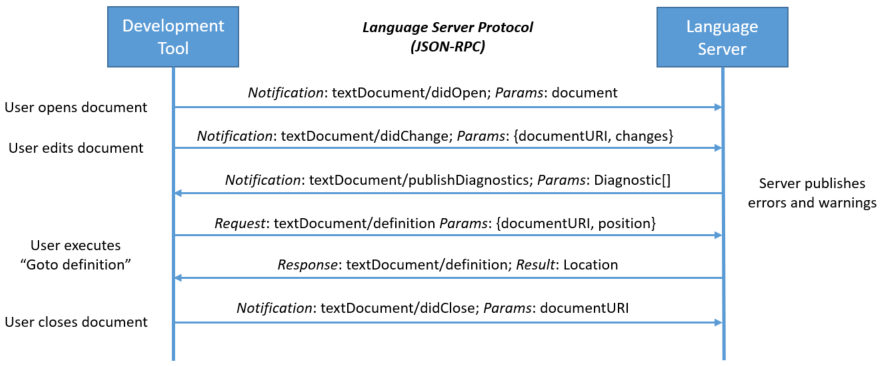
\includegraphics[height=0.3\linewidth]{Image/LSP-Diagram.png}
      \label{lsp-diagram}
      \footnotesize
      \\ Imagem não adaptada. \\
      Disponível em: \hyperlink{https://microsoft.github.io/language-server-protocol/overviews/lsp/overview/}{Microsoft - Language Server Protocol}
  \end{figure}
\end{frame}

\begin{frame}{Language Server Protocol - Instalação e Configuração}
  \textbf{Suporte nativo da API}
    \begin{columns}
      \begin{column}{0.4\textwidth}
        \begin{figure}
            \centering
            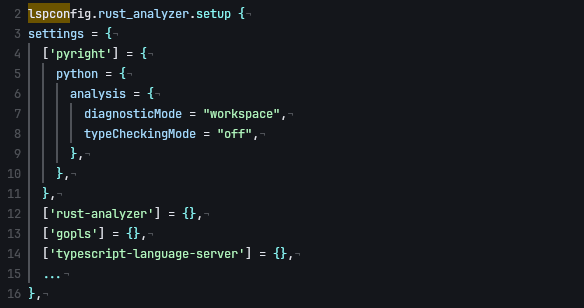
\includegraphics[height=0.6\linewidth]{Image/nvim-lspconfig.png}
            \label{nvim-lspconfig}
        \end{figure}
      \end{column}

      \begin{column}{0.6\textwidth}
        \begin{widedescription}
          \item Além de oferecer \textit{bindinds} nativas para a comunicação com LSPs, a configuração dos clientes pode
            ser feita de forma simples e direta através do pacote \texttt{nvim-lspconfig}
        \end{widedescription}
      \end{column}
  \end{columns}
\end{frame}

\begin{frame}{Language Server Protocol - Instalação e Configuração}
  \textbf{\texttt{nvim-lspconfig} + \texttt{Mason.nvim} = Configuração rápida, fácil, e portátil}
  \begin{figure}
      \centering
      
\includegraphics[height=0.3\linewidth]{Image/Mason-Logo.png}
      \label{mason-logo}
      \footnotesize
      \\ Imagem não adaptada. \\
      Disponível em:  \hyperlink{https://github.com/williamboman/mason.nvim}{Mason.nvim}
  \end{figure}
  \begin{quotation} \small
    Portable package manager for Neovim that runs everywhere Neovim runs. Easily install and manage LSP servers, DAP
    servers, linters, and formatters.\cite{masonNvim}
  \end{quotation}
\end{frame}

\begin{frame}{Language Server Protocol - Instalação e Configuração}
  \textbf{Um package-manager para servidores LSP}
  \begin{figure}
      \centering
      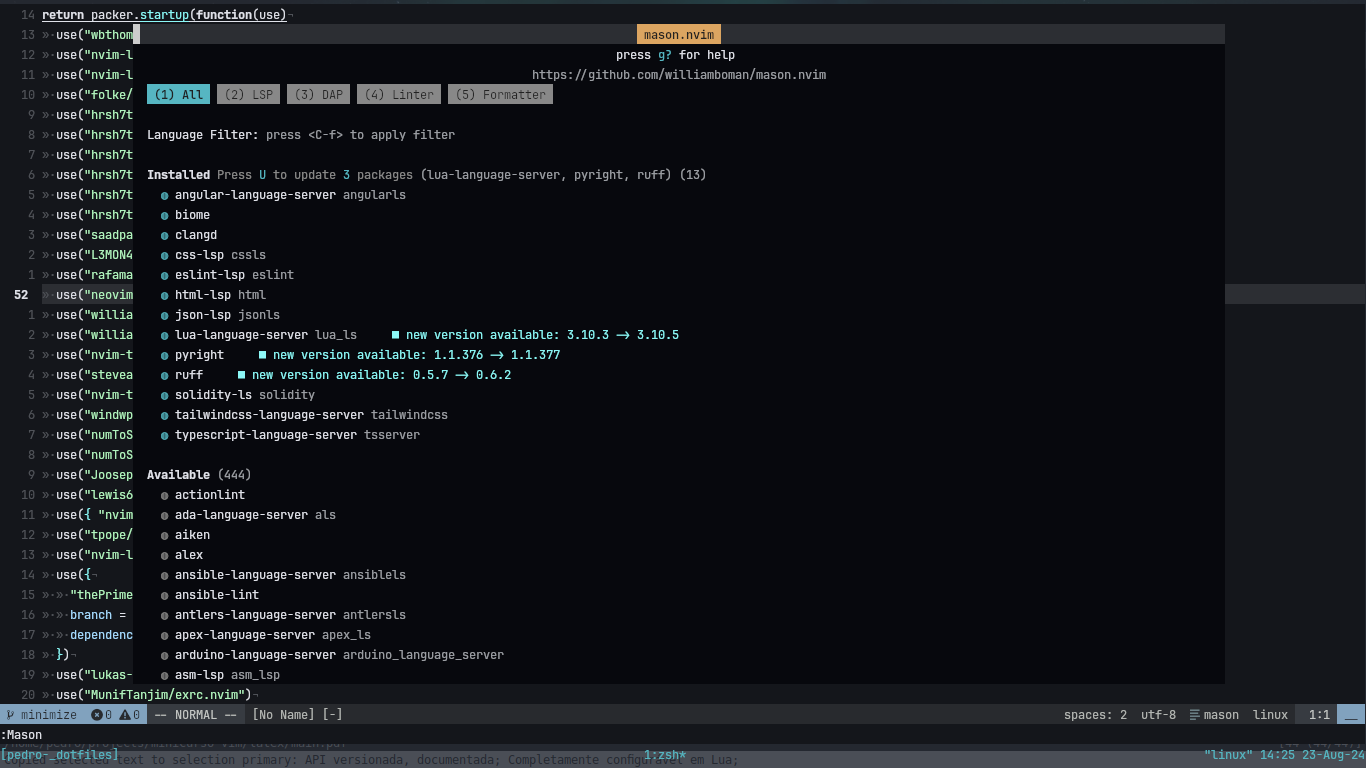
\includegraphics[height=0.5\linewidth]{Image/MasonLSP.png}
      \label{neovim-logo-2}
      \footnotesize
      \\ Instalação de LSPs via \textit{Mason.nvim} \\
  \end{figure}
\end{frame}

\begin{frame}{TreeSitter}
  \textbf{O motor sintático}
    \begin{columns}
      \begin{column}{0.3\textwidth}
        \begin{figure}
            \centering
            
\includegraphics[height=0.7\linewidth]{Image/TreeSitterLogo.png}
            \label{treesitter-logo}
        \end{figure}
      \end{column}

      \begin{column}{0.7\textwidth}
        \begin{widedescription}
          \item \begin{quotation} \small
            ``Tree-sitter is a parser generator tool and an incremental parsing library. It can build a
            concrete syntax tree for a source file and efficiently update the syntax tree as the source file is
            edited.''
          \end{quotation}
        \end{widedescription}
      \end{column}
  \end{columns}
\end{frame}

\begin{frame}{TreeSitter}
  \textbf{O motor sintático}
    \begin{widedescription}
      \item \textbf{General} enough to parse any programming language;
      \item \textbf{Fast} enough to parse on every keystroke in a text editor;
      \item \textbf{Robust} enough to provide useful results even in the presence of syntax errors;
      \item \textbf{Dependency-free} so that the runtime library (which is written in pure C) can be embedded in any application;
    \end{widedescription}
\end{frame}

\begin{frame}{TreeSitter}
  \textbf{O motor sintático}
    \begin{quotation} \small
      ``The goal of nvim-treesitter is both to provide a simple and easy way to use the interface for tree-sitter in
      Neovim and to provide some basic functionality such as highlighting based on it.''
    \end{quotation}
\end{frame}

\begin{frame}{TreeSitter}
  \textbf{O motor sintático}
  \begin{figure}
      \centering
      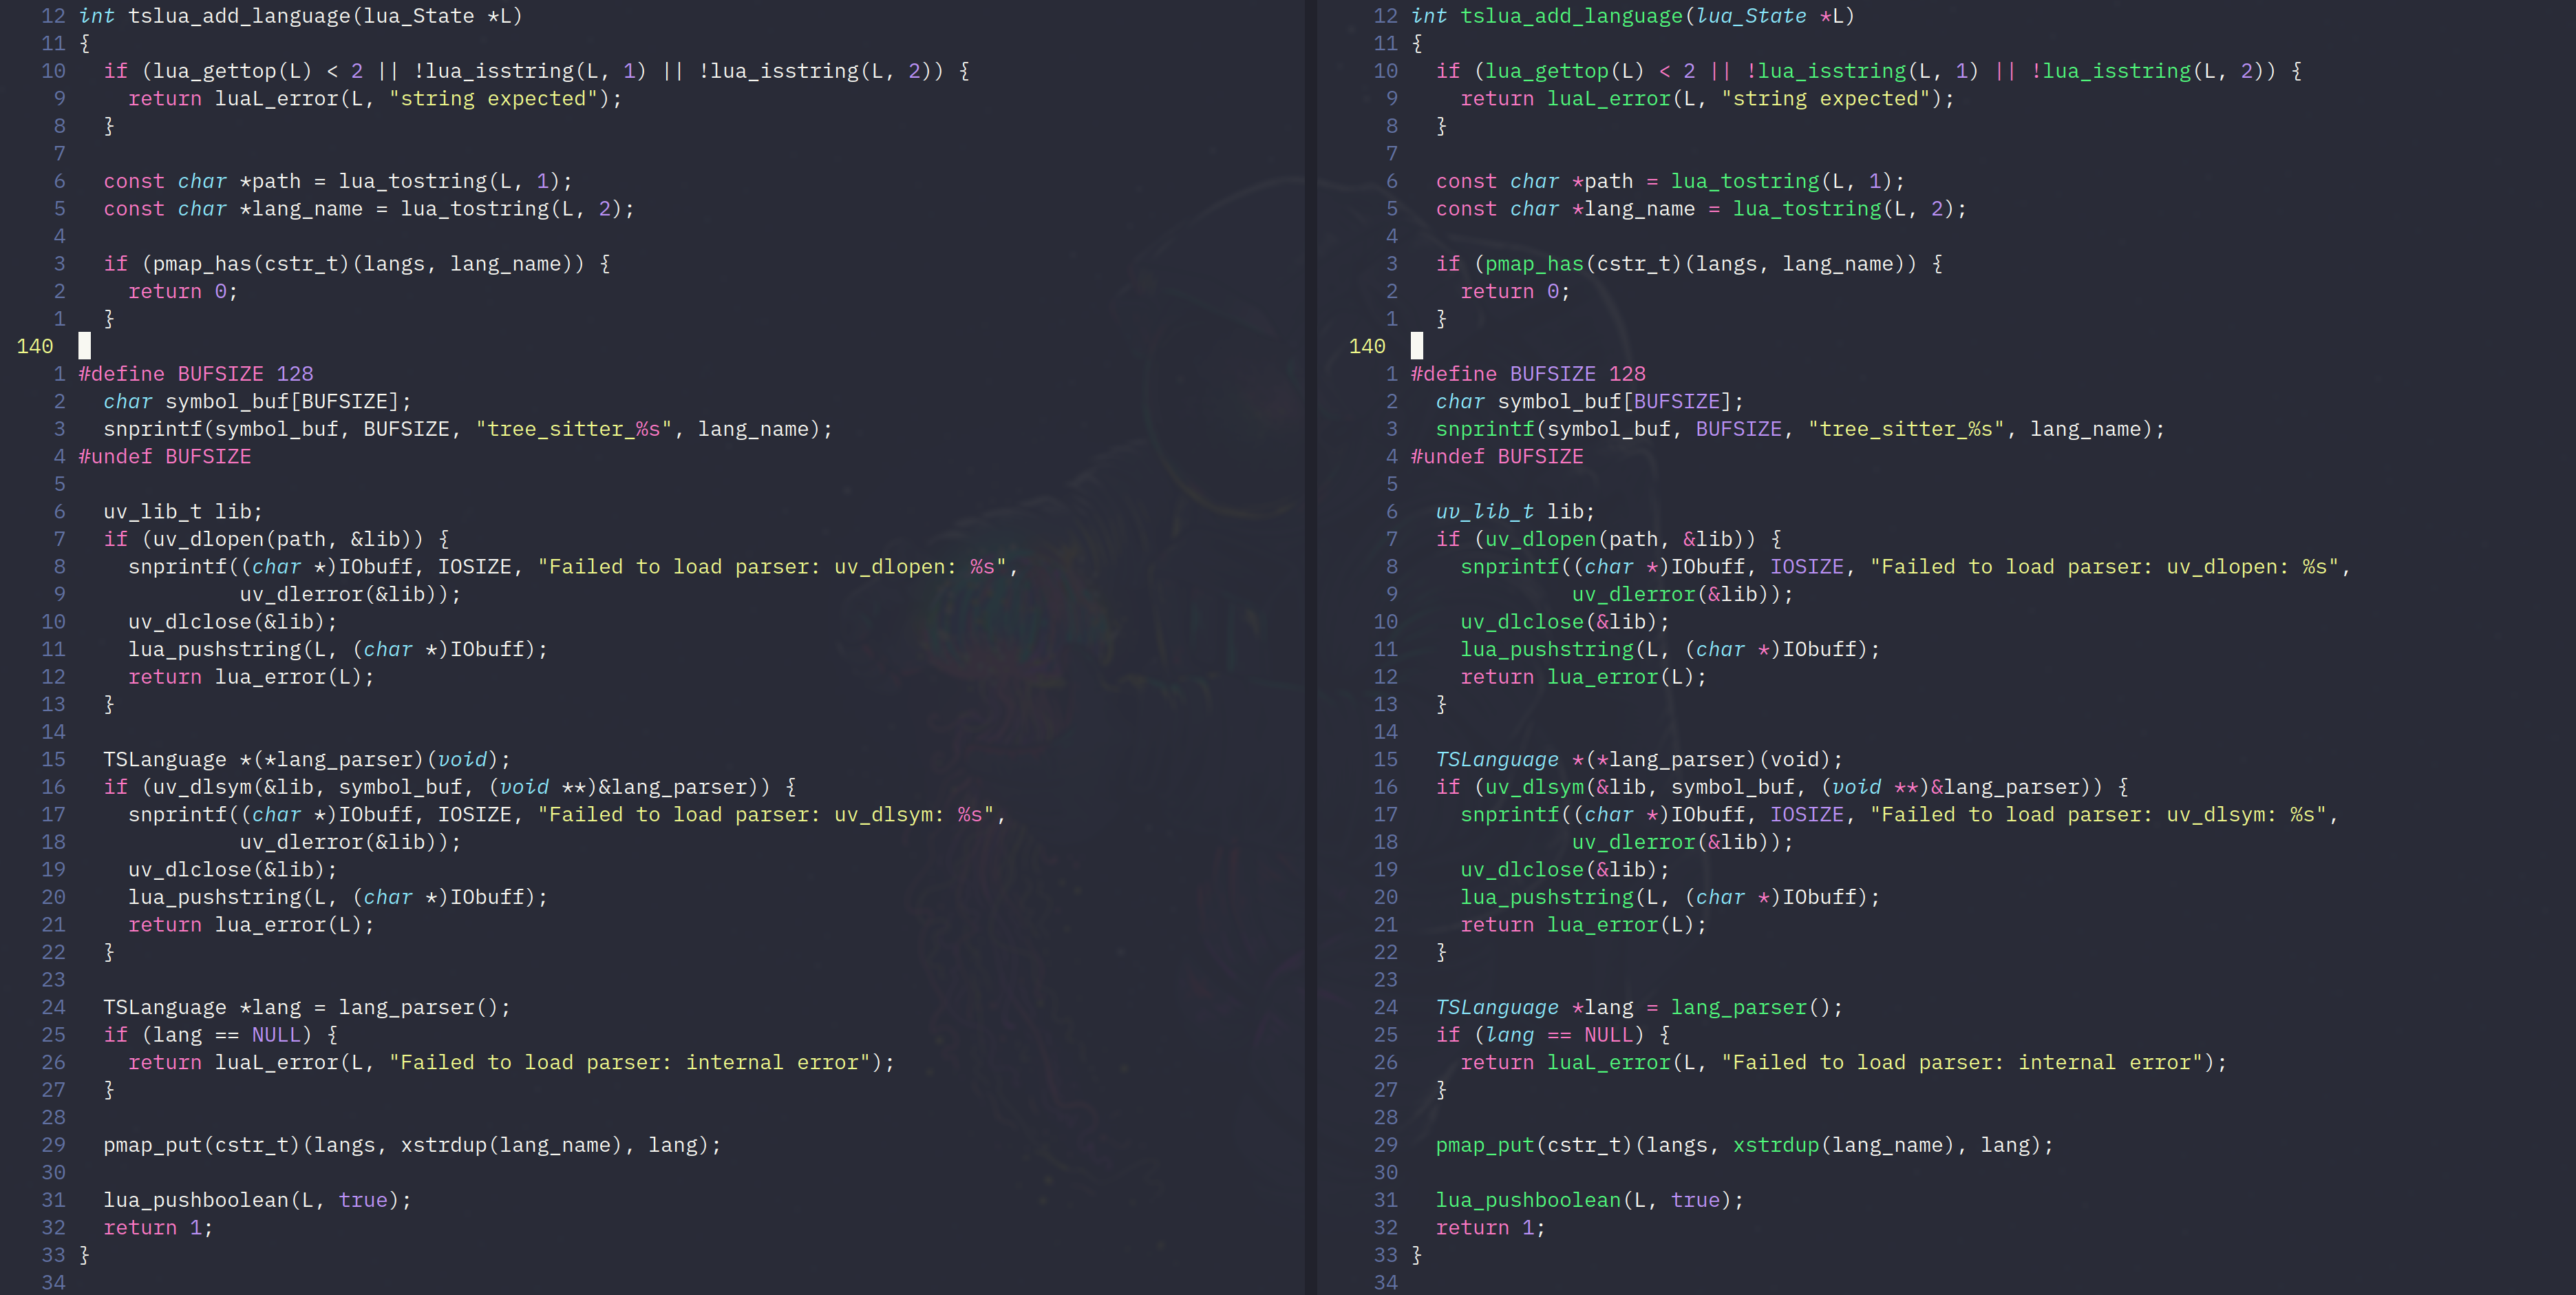
\includegraphics[height=0.5\linewidth]{Image/TreeSitter-Highlighting-Comparison.png}
      \label{treesitter-syntax-highlighting}
      \footnotesize
      \\ \textit{Highlighting} de sintaxe através da árvore construída\\
  \end{figure}
\end{frame}

\begin{frame}{TreeSitter}
  \textbf{O motor sintático}
  \begin{figure}
      \centering
      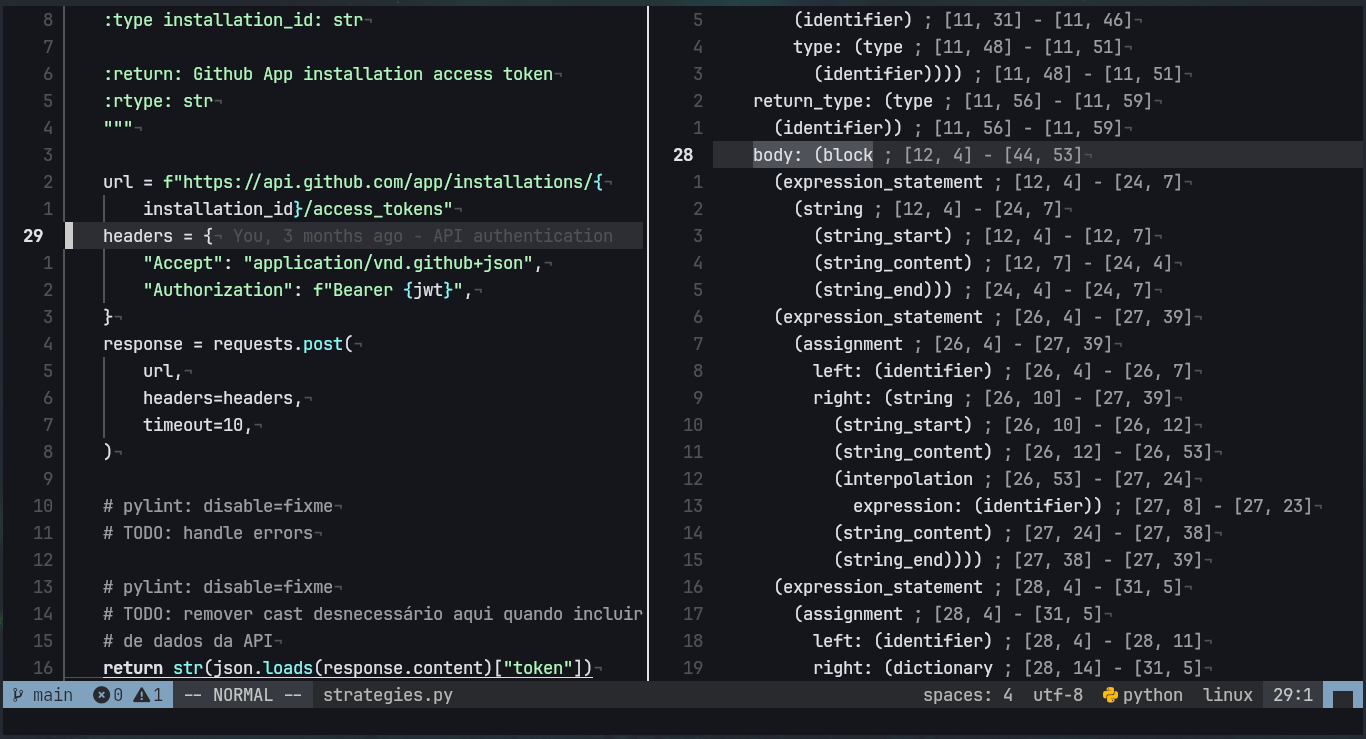
\includegraphics[height=0.5\linewidth]{Image/InspectTree.png}
      \label{treesitter-inspect-tree}
      \footnotesize
      \\ A ferramenta permite inspecionar a estrutura da árvore sintática em tempo real \\
  \end{figure}
\end{frame}

\begin{frame}{Plugins}
  \textbf{Plugin managers}
    \begin{widedescription}
      \item \texttt{pathogen}
      \item \texttt{vundle}
      \item \texttt{vim-plug}
      \item \texttt{packer.nvim}
      \item \textbf{\texttt{lazy.nvim}}
    \end{widedescription}
\end{frame}

\begin{frame}{Plugins}
  \textbf{Plugin managers}
  \begin{figure}
      \centering
      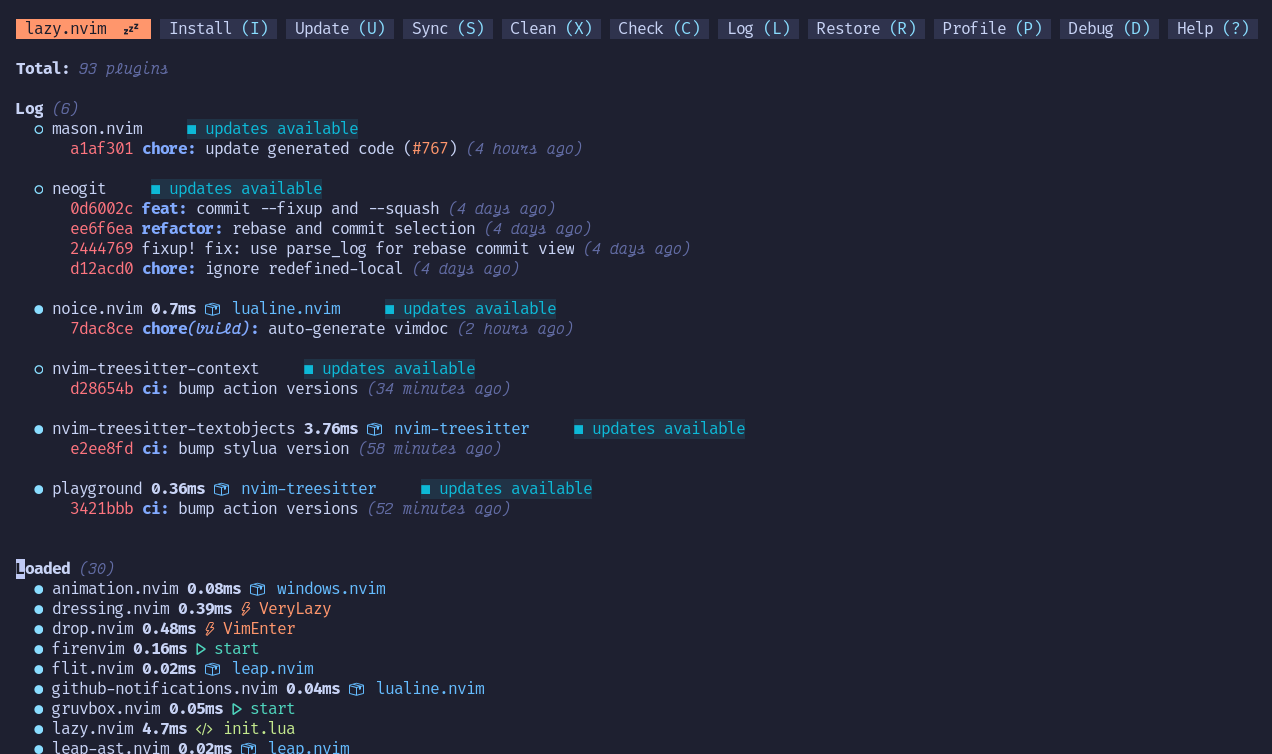
\includegraphics[height=0.5\linewidth]{Image/LazyVim.png}
      \label{lazy-vim}
      \footnotesize
      \\ Instalação interativa de plugins com \texttt{lazy.nvim} \\
  \end{figure}
\end{frame}

\begin{frame}{Lua}
  \textbf{Brasil mentioned!?!?!?}
  \begin{figure}
      \centering
      
\includegraphics[height=0.4\linewidth]{Image/Lua-Logo.png}
      \label{lua-logo}
      \footnotesize
      \\ Imagem não adaptada. \\
      Disponível em:  \hyperlink{https://www.lua.org/}{www.lua.org}
  \end{figure}
\end{frame}

\begin{frame}{Lua}
  \textbf{API}
    \begin{widedescription}
        \item The "Vim API" inherited from Vim: Ex-commands and builtin-functions as
          well as user-functions in Vimscript. These are accessed through \texttt{vim.cmd()}
          and \texttt{vim.fn} respectively.
        \item The "Nvim API" written in C for use in remote plugins and GUIs; see api.
          These functions are accessed through \texttt{vim.api}.
    \end{widedescription}
\end{frame}
